\documentclass[aspectratio=169, 10pt]{beamer}

% =========================================================
% PAQUETES Y CONFIGURACIÓN LINGÜÍSTICA
% =========================================================
\usepackage{polyglossia}
\setmainlanguage{spanish}
\usepackage{fontspec}
\usepackage{amsmath, amssymb, amsfonts}
\usepackage{graphicx}
\usepackage{booktabs}
\usepackage{tabularx}
\usepackage{colortbl}
\usepackage{tikz}
\usetikzlibrary{shapes.geometric, arrows.meta, positioning, calc, shadows}
\usepackage[most]{tcolorbox}
\usepackage{caption}
\usepackage{subcaption}

% =========================================================
% PALETA DE COLORES (DARK NAVY THEME - ESTILO SLATE UPP)
% =========================================================
\definecolor{bgNavy}{HTML}{101E2E}        % Fondo principal
\definecolor{cardNavy}{HTML}{1A293B}      % Tarjetas/Bloques
\definecolor{cardBorder}{HTML}{334155}    % Borde suave
\definecolor{purpleUPP}{HTML}{701445}      % Color Institucional UPP
\definecolor{purpleAccent}{HTML}{8B5CF6}   % Púrpura brillante
\definecolor{cyanAccent}{HTML}{06B6D4}     % Cian tecnológico
\definecolor{emeraldAccent}{HTML}{10B981}  % Verde éxito
\definecolor{amberAccent}{HTML}{F59E0B}    % Ámbar alerta
\definecolor{textWhite}{HTML}{F8FAFC}      % Texto blanco brillante
\definecolor{textMuted}{HTML}{94A3B8}      % Texto secundario gris

% Configuración global de colores en Beamer
\setbeamercolor{background canvas}{bg=bgNavy}
\setbeamercolor{normal text}{fg=textWhite}
\setbeamercolor{frametitle}{fg=textWhite, bg=cardNavy}
\setbeamercolor{title}{fg=textWhite}
\setbeamercolor{subtitle}{fg=cyanAccent}
\setbeamercolor{author}{fg=textMuted}
\setbeamercolor{date}{fg=textMuted}
\setbeamercolor{item}{fg=cyanAccent}
\setbeamercolor{subitem}{fg=purpleAccent}
\setbeamercolor{section in toc}{fg=textWhite}
\setbeamercolor{subsection in toc}{fg=textMuted}

% Desactivar barra de navegación Beamer por defecto
\setbeamertemplate{navigation symbols}{}

% =========================================================
% PLANTILLAS DE ENCABEZADO Y PIE DE PÁGINA
% =========================================================
\setbeamertemplate{frametitle}{
    \nointerlineskip
    \begin{beamercolorbox}[wd=\paperwidth, ht=1.2cm, dp=0.3cm, leftskip=0.8cm, rightskip=0.8cm]{frametitle}
        \usebeamerfont{frametitle}\insertframetitle
        \vskip0.1cm
        \hrule height 1.5pt width \textwidth color cyanAccent
    \end{beamercolorbox}
}

\setbeamertemplate{footline}{
    \begin{beamercolorbox}[wd=\paperwidth, ht=0.5cm, dp=0.2cm, leftskip=0.8cm, rightskip=0.8cm]{author in head/foot}
        \fontsize{7pt}{8pt}\selectfont
        \color{textMuted}
        \insertshorttitle \ \ \textbf{|} \ \ UPP -- Ingeniería en Software
        \hfill
        Diapositiva \insertframenumber{} de \inserttotalframenumber
    \end{beamercolorbox}
}

% =========================================================
% BLOQUES PERSONALIZADOS (TCOLORBOX)
% =========================================================
\newtcolorbox{darkcard}[1][]{
    colback=cardNavy,
    colframe=cardBorder,
    coltitle=textWhite,
    fonttitle=\bfseries\small,
    arc=4pt,
    boxrule=0.8pt,
    left=6pt, right=6pt, top=6pt, bottom=6pt,
    #1
}

\newtcolorbox{metriccard}[2][]{
    colback=cardNavy,
    colframe=purpleAccent,
    title=#2,
    coltitle=textWhite,
    fonttitle=\bfseries\scriptsize,
    arc=4pt,
    boxrule=1pt,
    left=4pt, right=4pt, top=4pt, bottom=4pt,
    #1
}

\newtcolorbox{accentcard}[2][]{
    colback=cardNavy,
    colframe=cyanAccent,
    title=#2,
    coltitle=textWhite,
    fonttitle=\bfseries\scriptsize,
    arc=4pt,
    boxrule=1pt,
    left=4pt, right=4pt, top=4pt, bottom=4pt,
    #1
}

% =========================================================
% DATOS DE LA PRESENTACIÓN
% =========================================================
\title[Optimización de Rutas UPP via UCB1]{Optimización Inteligente de Rutas de Transporte UPP mediante Regresión OLS y UCB1 Multi-Armed Bandit}
\subtitle{Proyecto Final de Inteligencia Artificial -- Cuatrimestre Mayo-Agosto 2026}
\author{Equipo de Desarrollo UPP}
\institute{Universidad Politécnica de Pachuca -- Ingeniería en Software}
\date{20 de Agosto de 2026}

% =========================================================
% INICIO DEL DOCUMENTO
% =========================================================
\begin{document}

% ---------------------------------------------------------
% DIAPOSITIVA 1: PORTADA
% ---------------------------------------------------------
\begin{frame}[plain]
    \vfill
    \begin{darkcard}[colframe=purpleUPP, boxrule=1.5pt]
        \begin{columns}[c]
            \begin{column}{0.15\textwidth}
                \centering
                \IfFileExists{logos/UPP_logo.png}{
\includegraphics[height=1.2cm]{logos/UPP_logo.png}}{}
            \end{column}
            \begin{column}{0.66\textwidth}
                \centering
                \fontsize{12pt}{14pt}\selectfont \textbf{\color{textWhite}{UNIVERSIDAD POLITÉCNICA DE PACHUCA}}\\[2pt]
                \fontsize{9pt}{11pt}\selectfont \color{cyanAccent}{Programa Educativo de Ingeniería en Software}\\[2pt]
                \fontsize{8pt}{10pt}\selectfont \color{textMuted}{Asignatura: Inteligencia Artificial}
            \end{column}
            \begin{column}{0.15\textwidth}
                \centering
                \IfFileExists{logos/SOFT_logo.png}{
\includegraphics[height=1.2cm]{logos/SOFT_logo.png}}{}
            \end{column}
        \end{columns}
    \end{darkcard}
    \vskip0.2cm
    
    \begin{darkcard}[colframe=cyanAccent, boxrule=1.2pt]
        \centering
        \fontsize{13pt}{16pt}\selectfont \textbf{\color{textWhite}{Optimización de Rutas UPP via UCB1 Multi-Armed Bandit}}\\[4pt]
        \fontsize{9pt}{11pt}\selectfont \color{textMuted}{Modelo Predictivo OLS y Aprendizaje por Refuerzo para Despacho Dinámico}
    \end{darkcard}
    \vskip0.2cm

    \begin{darkcard}[colframe=cardBorder]
        \fontsize{8pt}{10pt}\selectfont
        \begin{columns}[T]
            \begin{column}{0.5\textwidth}
                \textbf{\color{cyanAccent}{Integrantes del Equipo:}}\\[2pt]
                \color{textWhite}{Emmanuel \& Equipo de Desarrollo IA UPP}
            \end{column}
            \begin{column}{0.5\textwidth}
                \textbf{\color{cyanAccent}{Asistencia de IA:}}\\[2pt]
                \color{emeraldAccent}{\textbf{Asistencia de IA: Google Gemini \& OpenAI Codex}}
            \end{column}
        \end{columns}
    \end{darkcard}
    \vfill
\end{frame}

% ---------------------------------------------------------
% DIAPOSITIVA 2: AGENDA
% ---------------------------------------------------------
\begin{frame}{Agenda y Estructura del Proyecto}
    \begin{columns}[T]
        \begin{column}{0.5\textwidth}
            \begin{darkcard}[title=\color{cyanAccent}{Parte I: Fundamentos y Simulación}]
                \begin{enumerate}
                    \item \textbf{Definición del Problema:} Cuello de botella en la ruta UPP -- Puente de Tuzos.
                    \item \textbf{Dataset Simulado:} Proceso estocástico Poisson ($\lambda$ variable por franja).
                    \item \textbf{Modelo Predictivo OLS:} Regresión lineal simple y estimadores MCO.
                \end{enumerate}
            \end{darkcard}
        \end{column}
        \begin{column}{0.5\textwidth}
            \begin{darkcard}[title=\color{purpleAccent}{Parte II: Prescripción y Resultados}]
                \begin{enumerate}\setcounter{enumii}{3}
                    \item \textbf{Algoritmo UCB1:} Multi-Armed Bandit para despacho adaptativo.
                    \item \textbf{Resultados Experimentales:} Comparativa $a_0$ (Política Tradicional) vs UCB1.
                    \item \textbf{Bitácora de IA \& Conclusiones:} Aprendizaje crítico y recomendaciones.
                \end{enumerate}
            \end{darkcard}
        \end{column}
    \end{columns}
\end{frame}

% ---------------------------------------------------------
% DIAPOSITIVA 3: DEFINICIÓN DEL PROBLEMA
% ---------------------------------------------------------
\begin{frame}{Definición del Problema y Contexto UPP}
    \begin{columns}[T]
        \begin{column}{0.58\textwidth}
            \begin{darkcard}[title=\color{cyanAccent}{La Problemática Operativa}]
                \begin{itemize}
                    \item \textbf{Política Tradicional ($a_0$):} Salir únicamente cuando la unidad alcanza el cupo total de \textbf{18 pasajeros}.
                    \item \textbf{Incapacidad Adaptativa:} En horas valle (10:00--12:00 y 16:00--18:00), la tasa de llegada de alumnos decae drásticamente.
                    \item \textbf{Consecuencia:} Tiempos de espera que superan los \textbf{60--80 minutos}, generando hacinamiento y colapso de satisfacción estudiantil.
                \end{itemize}
            \end{darkcard}
        \end{column}
        \begin{column}{0.4\textwidth}
            \begin{metriccard}{Objetivo de Optimización}
                \fontsize{8.5pt}{11pt}\selectfont
                Transicionar de una regla estática rígida a un \textbf{sistema de decisión dinámico} que maximice la ocupación vehicular minimizando el tiempo acumulado de espera estudiantil.
            \end{metriccard}
            \vskip0.1cm
            \begin{accentcard}{Rutas Monitoreadas}
                \begin{itemize}
                    \item \textbf{Puente de Tuzos:} Llegada Poisson $\approx 1$ pax / 7 min.
                    \item \textbf{San Agustín:} Llegada Poisson $\approx 1$ pax / 10 min.
                \end{itemize}
            \end{accentcard}
        \end{column}
    \end{columns}
\end{frame}

% ---------------------------------------------------------
% DIAPOSITIVA 4: DATASET SIMULADO
% ---------------------------------------------------------
\begin{frame}{Dataset Simulado de Demanda y Despachos}
    \begin{columns}[T]
        \begin{column}{0.5\textwidth}
            \begin{darkcard}[title=\color{cyanAccent}{Generación de Demanda Poisson}]
                \begin{equation*}
                    P(X=k) = \frac{\lambda^k e^{-\lambda}}{k!}
                \end{equation*}
                \begin{itemize}
                    \item \textbf{Hora Pico (07:00-09:00, 13:00-15:00):} $\lambda_{\text{pico}} = 3.5$ alumnos / 15 min.
                    \item \textbf{Hora Valle (10:00-12:00, 16:00-18:00):} $\lambda_{\text{valle}} = 1.2$ alumnos / 15 min.
                    \item \textbf{Periodo Evaluado:} 21 días de operación ($1,466$ despachos registrados).
                \end{itemize}
            \end{darkcard}
        \end{column}
        \begin{column}{0.5\textwidth}
            \begin{darkcard}[title=\color{purpleAccent}{Estructura del Dataset (13 Columnas)}]
                \fontsize{7.5pt}{9.5pt}\selectfont
                \begin{tabularx}{\textwidth}{l X}
                    \toprule
                    \textbf{Columna} & \textbf{Descripción} \\
                    \midrule
                    \texttt{fecha, hora\_intervalo} & Marca temporal del despacho. \\
                    \texttt{ruta} & Puente de Tuzos / San Agustín. \\
                    \texttt{alumnos\_esperando} & Cola inicial al llegar la combi ($X$). \\
                    \texttt{llegadas\_intervalo} & Alumnos llegados durante espera. \\
                    \texttt{pasajeros\_al\_salir} & Pasajeros a bordo al despachar. \\
                    \texttt{tiempo\_espera\_acum} & Tiempo total transcurrido ($Y$). \\
                    \texttt{tipo\_salida} & Llena ($18$ pax) / Parcial ($<18$). \\
                    \bottomrule
                \end{tabularx}
            \end{darkcard}
        \end{column}
    \end{columns}
\end{frame}

% ---------------------------------------------------------
% DIAPOSITIVA 5: REGRESIÓN LINEAL OLS (TEORÍA)
% ---------------------------------------------------------
\begin{frame}{Modelo de Regresión Lineal Simple (OLS)}
    \begin{columns}[T]
        \begin{column}{0.5\textwidth}
            \begin{darkcard}[title=\color{cyanAccent}{Formulación Matemática OLS}]
                Se evalúa la relación entre la cola inicial ($X$) y los minutos requeridos para despachar ($Y$):
                \begin{equation*}
                    Y_i = a + b \cdot X_i + e_i
                \end{equation*}
                \textbf{Estimadores de Mínimos Cuadrados Ordinarios:}
                \begin{equation*}
                    b = \frac{\sum (X_i - \bar{X})(Y_i - \bar{Y})}{\sum (X_i - \bar{X})^2}, \quad a = \bar{Y} - b \bar{X}
                \end{equation*}
            \end{darkcard}
        \end{column}
        \begin{column}{0.5\textwidth}
            \begin{darkcard}[title=\color{purpleAccent}{Hipótesis Estadísticas Evaluadas}]
                \begin{itemize}
                    \item \textbf{Hipótesis Nula ($H_0: b = 0$):} La cantidad de alumnos en espera no influye en los minutos de despacho.
                    \item \textbf{Hipótesis Alternativa ($H_1: b \neq 0$):} Existe relación lineal significativa entre la cola inicial y el tiempo restante.
                \end{itemize}
            \end{darkcard}
        \end{column}
    \end{columns}
\end{frame}

% ---------------------------------------------------------
% DIAPOSITIVA 6: RESULTADOS REGRESIÓN OLS
% ---------------------------------------------------------
\begin{frame}{Resultados y Ajuste de Regresión OLS}
    \begin{columns}[T]
        \begin{column}{0.48\textwidth}
            \begin{darkcard}[title=\color{cyanAccent}{Ecuación Estimada y Métricas}]
                \begin{equation*}
                    \widehat{Y} = 14.1068 - 2.5395 X
                \end{equation*}
                \fontsize{8pt}{10pt}\selectfont
                \begin{itemize}
                    \item \textbf{Intercepto ($a = 14.11$ min):} Tiempo promedio estimado al llegar sin alumnos en cola ($X=0$).
                    \item \textbf{Pendiente ($b = -2.54$ min/pax):} Cada alumno adicional en cola reduce en $2.54$ min el tiempo para salir.
                    \item \textbf{Coeficiente $R^2 = 0.121$ ($12.1\%$):} Significativo ($p = 5.83 \times 10^{-43} < 0.001, F = 201.8$).
                \end{itemize}
            \end{darkcard}
        \end{column}
        \begin{column}{0.5\textwidth}
            \begin{center}
                \IfFileExists{../outputs/plots/fig1_regresion.png}{
                    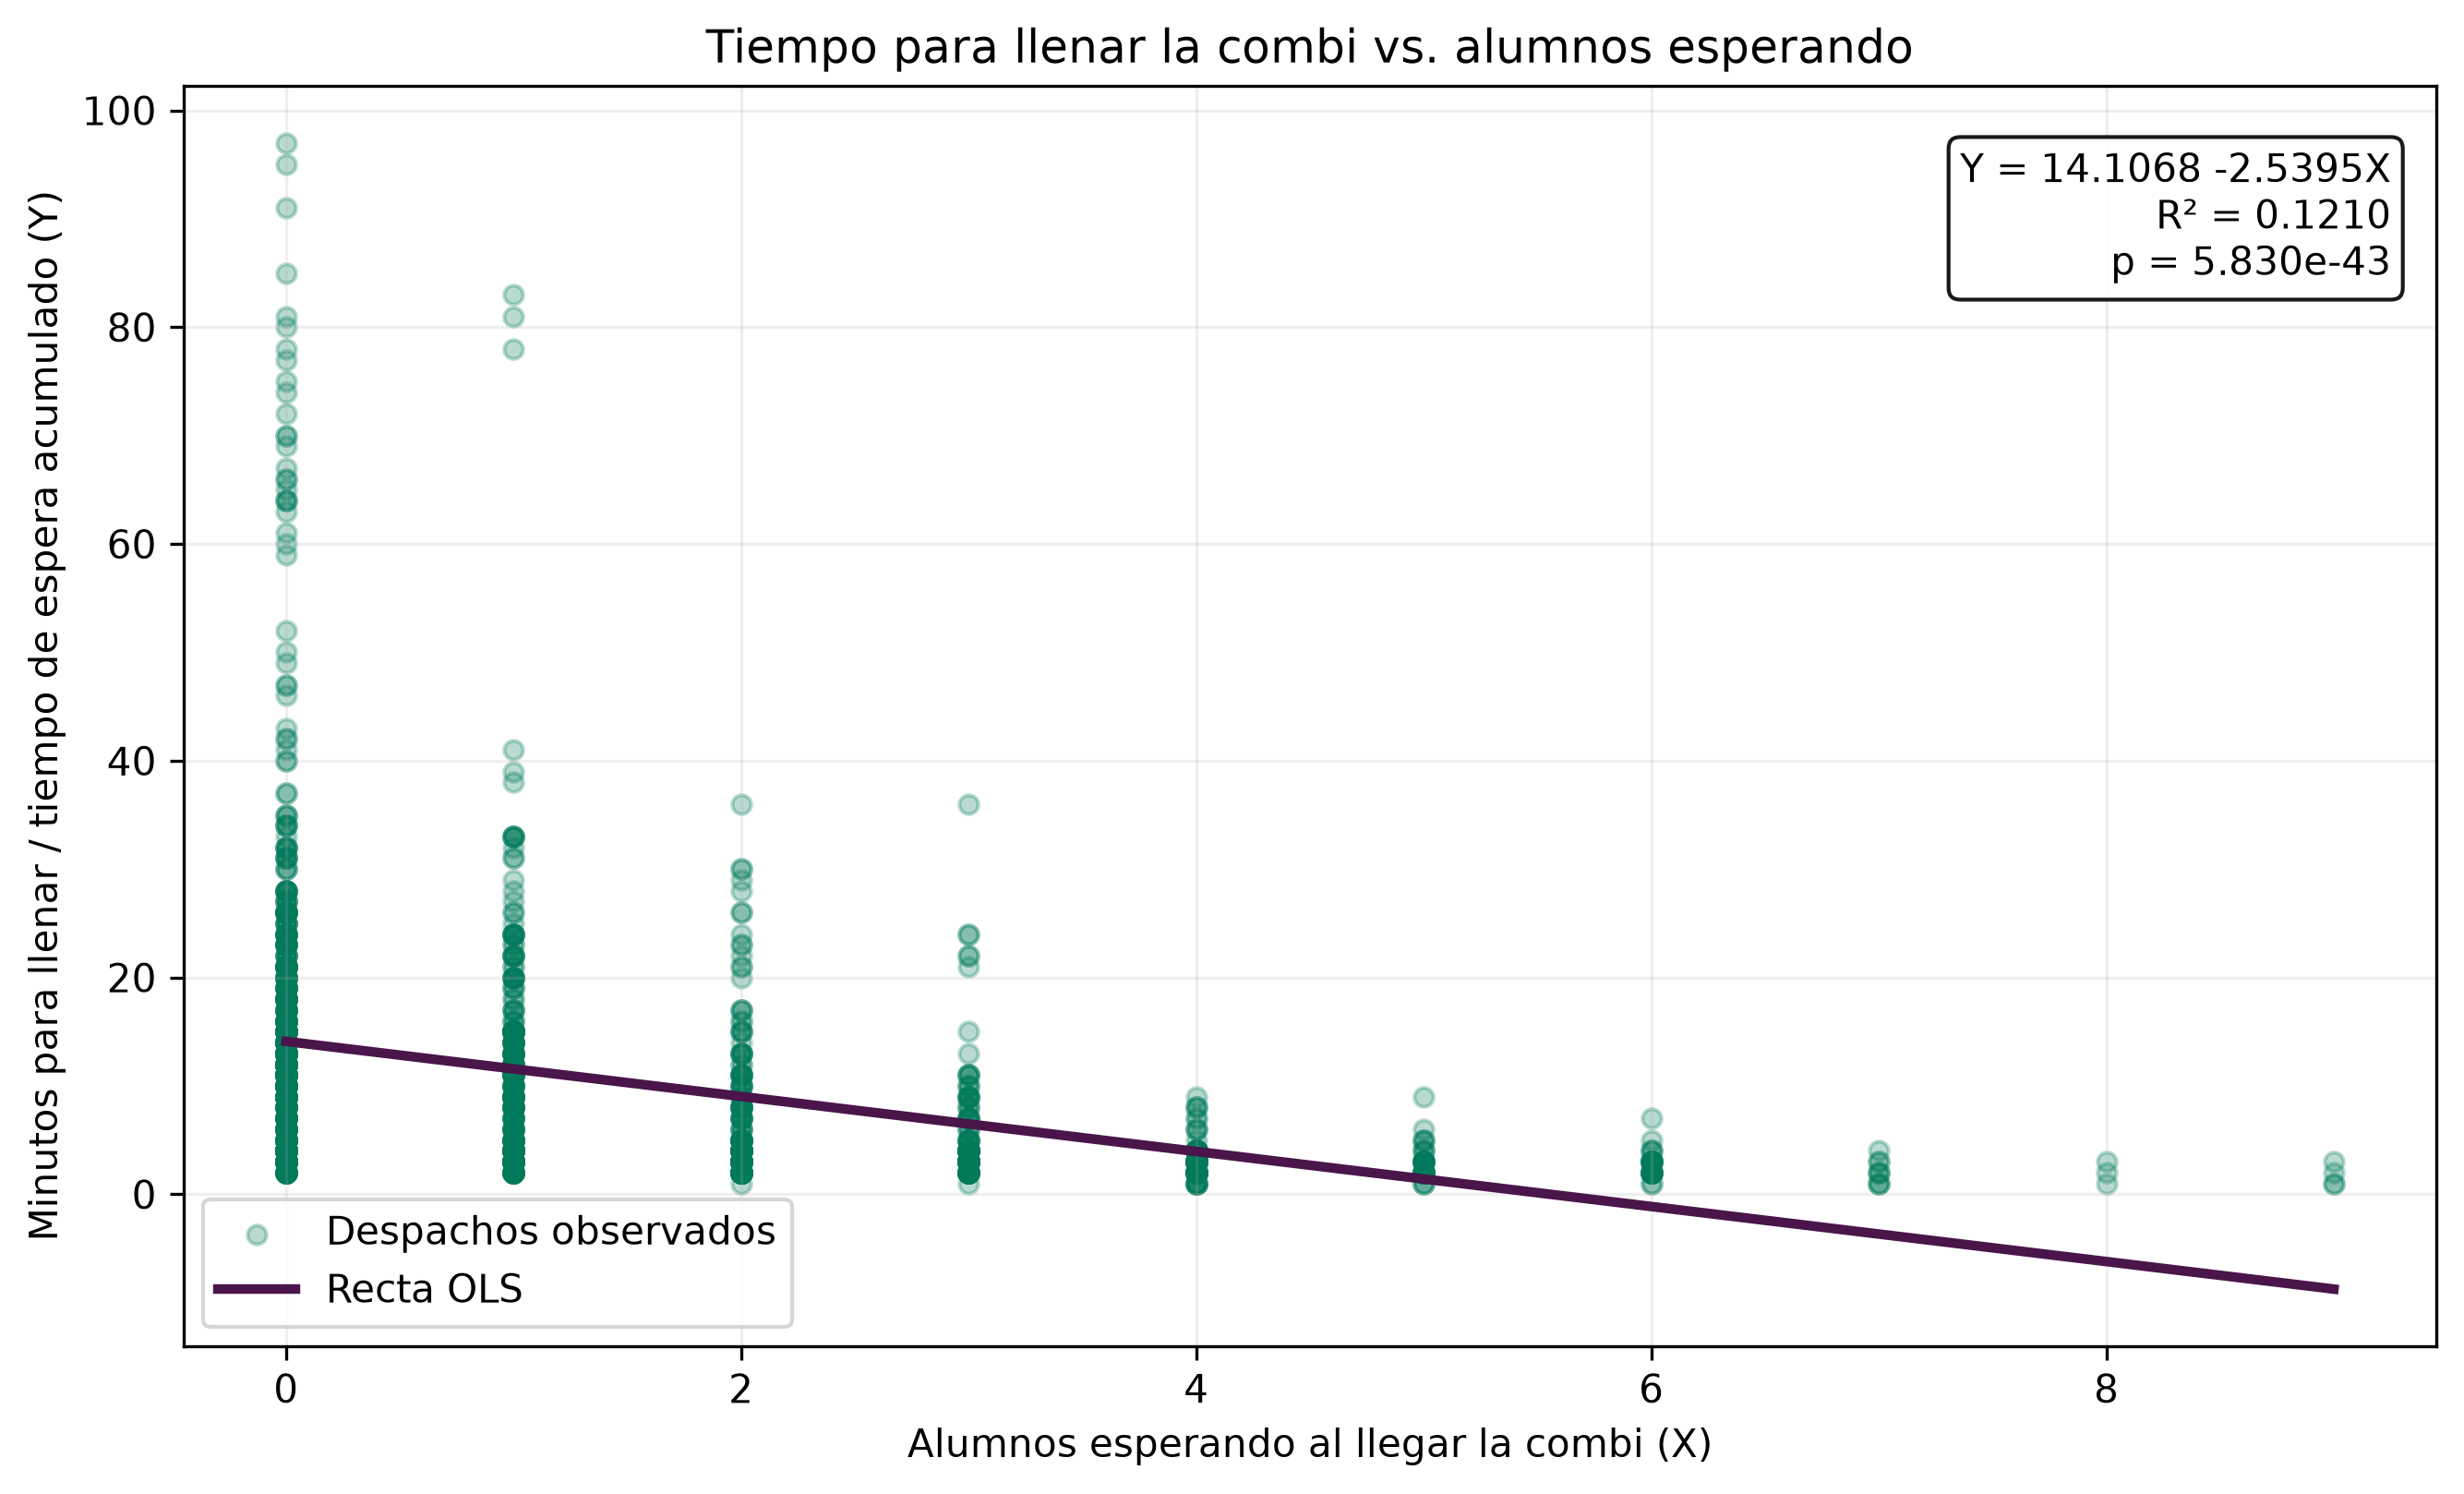
\includegraphics[height=4.8cm, width=\textwidth, keepaspectratio]{../outputs/plots/fig1_regresion.png}
                }{
                    \color{textMuted}{[Gráfica OLS Ajustada]}
                }
            \end{center}
        \end{column}
    \end{columns}
\end{frame}

% ---------------------------------------------------------
% DIAPOSITIVA 7: PRUEBAS DE SUPUESTOS OLS
% ---------------------------------------------------------
\begin{frame}{Verificación de Supuestos Estadísticos OLS}
    \begin{columns}[T]
        \begin{column}{0.48\textwidth}
            \begin{darkcard}[title=\color{cyanAccent}{Diagnóstico de Supuestos}]
                \fontsize{8pt}{10pt}\selectfont
                \begin{itemize}
                    \item \textbf{Linealidad:} Test cuadrático $F=25.86, p < 0.001$. Curvatura menor detectada en horas valle.
                    \item \textbf{Independencia (Durbin-Watson):} $DW = 1.6002 \in [1.5, 2.5]$, confirmando ausencia de autocorrelación severa.
                    \item \textbf{Homocedasticidad (Breusch-Pagan):} $LM = 25.79, p < 0.001$. Heterocedasticidad presente debido a la variación de demanda.
                \end{itemize}
            \end{darkcard}
        \end{column}
        \begin{column}{0.5\textwidth}
            \begin{center}
                \IfFileExists{../outputs/plots/fig2_homocedasticidad.png}{
                    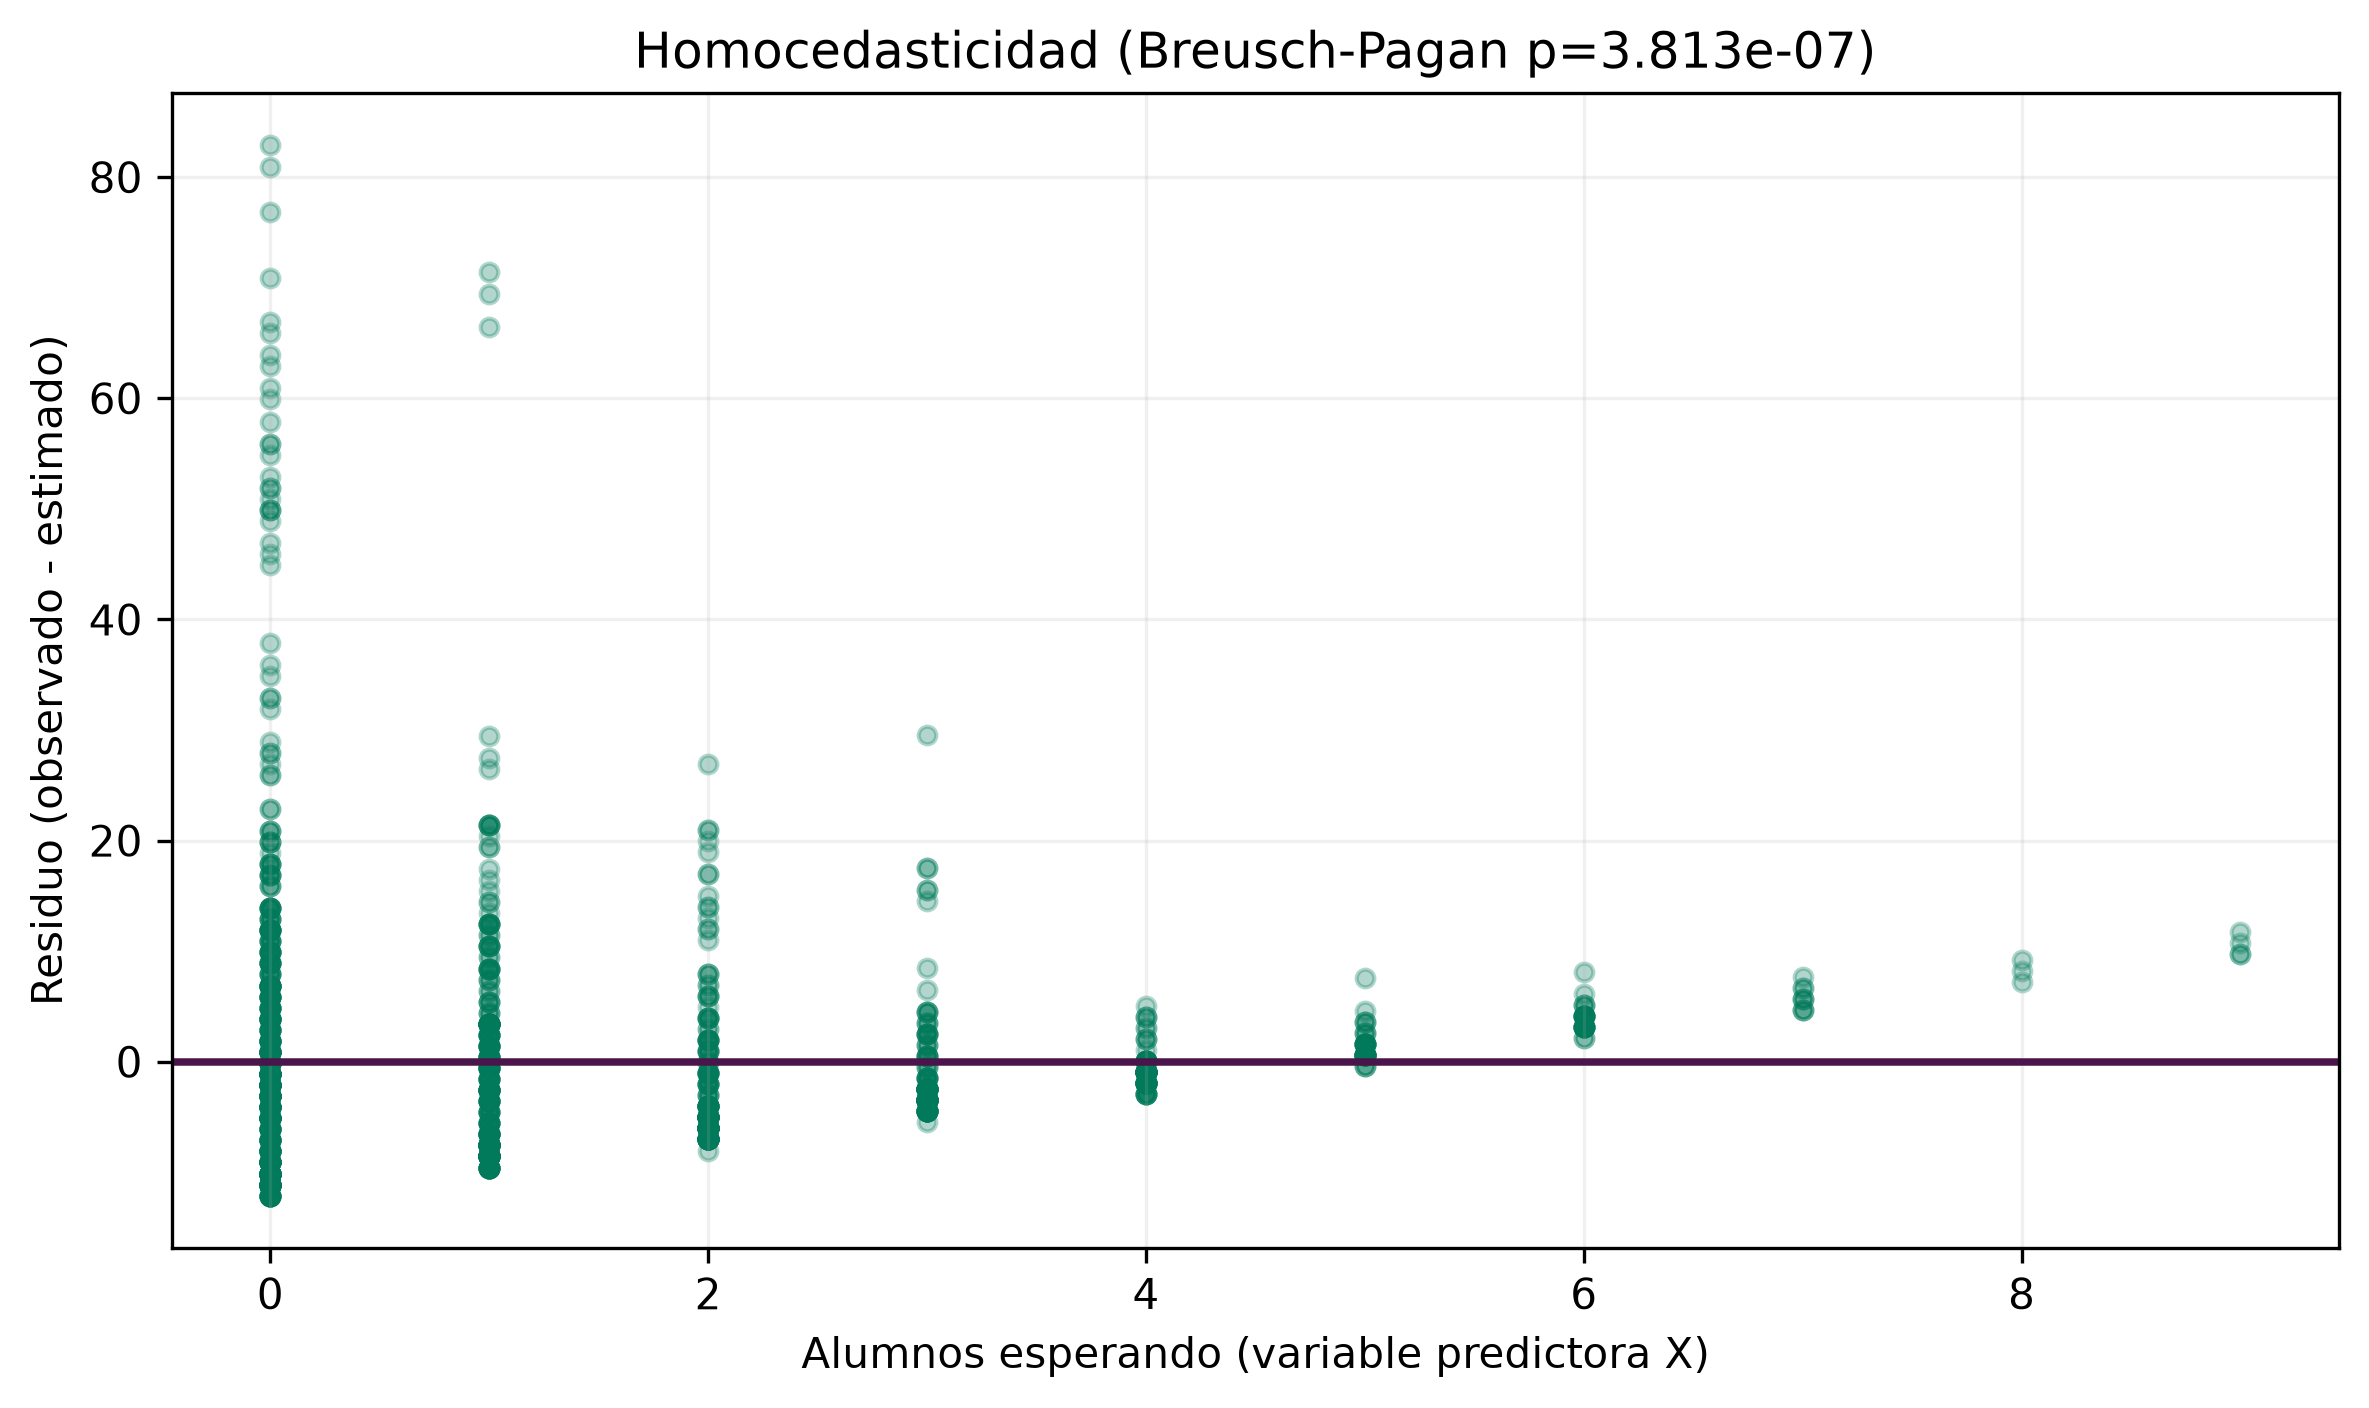
\includegraphics[height=4.8cm, width=\textwidth, keepaspectratio]{../outputs/plots/fig2_homocedasticidad.png}
                }{
                    \color{textMuted}{[Gráfica Homocedasticidad]}
                }
            \end{center}
        \end{column}
    \end{columns}
\end{frame}

% ---------------------------------------------------------
% DIAPOSITIVA 8: ALGORITMO UCB1 (TEORÍA)
% ---------------------------------------------------------
\begin{frame}{Aprendizaje por Refuerzo: Algoritmo UCB1}
    \begin{columns}[T]
        \begin{column}{0.5\textwidth}
            \begin{darkcard}[title=\color{cyanAccent}{Marco Multi-Armed Bandit}]
                El agente UCB1 equilibra la \textbf{explotación} del brazo con mayor recompensa observada y la \textbf{exploración} de brazos menos frecuentados:
                \begin{equation*}
                    A_t = \arg\max_{a} \left[ \bar{Q}_t(a) + c \sqrt{\frac{\ln t}{N_t(a)}} \right]
                \end{equation*}
                \fontsize{8pt}{10pt}\selectfont
                \begin{itemize}
                    \item $\bar{Q}_t(a)$: Recompensa promedio estimada del brazo $a$.
                    \item $N_t(a)$: Número de veces que se ha seleccionado el brazo $a$.
                    \item $c = \sqrt{2}$: Factor de exploración teóricamente óptimo.
                \end{itemize}
            \end{darkcard}
        \end{column}
        \begin{column}{0.5\textwidth}
            \begin{darkcard}[title=\color{purpleAccent}{Estado del Sistema en Cada Despacho}]
                \fontsize{8pt}{10pt}\selectfont
                \begin{itemize}
                    \item Hora y franja operativa (Pico / Valle).
                    \item Pasajeros actuales a bordo de la combi.
                    \item Tiempo transcurrido de espera en la terminal.
                    \item Predicción de demanda basada en regresión OLS.
                \end{itemize}
            \end{darkcard}
        \end{column}
    \end{columns}
\end{frame}

% ---------------------------------------------------------
% DIAPOSITIVA 9: CATÁLOGO DE BRAZOS UCB
% ---------------------------------------------------------
\begin{frame}{Catálogo de Políticas de Salida (Brazos UCB)}
    \begin{darkcard}[title=\color{cyanAccent}{Brazos Candidatos Evaluados por el Agente ($a_0 \dots a_4$)}]
        \centering
        \fontsize{8.5pt}{11pt}\selectfont
        \begin{tabularx}{\textwidth}{>{\bfseries\color{purpleAccent}}c l X c}
            \toprule
            \rowcolor{cardNavy!80!black}
            \textbf{Brazo} & \textbf{Identificador} & \textbf{Regla Operativa de Despacho} & \textbf{Tipo de Política} \\
            \midrule
            $a_0$ & \texttt{FullOnly} & Salir únicamente al alcanzar $18$ pasajeros. & Tradicional / Rígida \\
            $a_1$ & \texttt{Flex\_14p\_15m} & Salir con $\ge 14$ personas O tras 15 min de espera. & Dinámica Flexible \\
            $a_2$ & \texttt{Flex\_12p\_25m} & Salir con $\ge 12$ personas O tras 25 min de espera. & Dinámica Moderada \\
            $a_3$ & \texttt{Flex\_10p\_35m} & Salir con $\ge 10$ personas O tras 35 min de espera. & Dinámica Valle \\
            $a_4$ & \texttt{Flex\_8p\_45m} & Salir con $\ge 8$ personas O tras 45 min de espera. & Límite Máximo \\
            \bottomrule
        \end{tabularx}
    \end{darkcard}
\end{frame}

% ---------------------------------------------------------
% DIAPOSITIVA 10: FUNCIÓN DE RECOMPENSA NORMALIZADA
% ---------------------------------------------------------
\begin{frame}{Función de Recompensa Normalizada}
    \begin{columns}[T]
        \begin{column}{0.5\textwidth}
            \begin{darkcard}[title=\color{cyanAccent}{Cálculo de Penalización Multiobjetivo}]
                En cada decisión $t$, se evalúa la penalización global $P_t$:
                \begin{equation*}
                    P_t = w_1 \cdot \text{espera\_total} + w_2 \cdot \text{alumnos\_dejados} + w_3 \cdot \text{asientos\_vacíos}
                \end{equation*}
                \fontsize{8pt}{10pt}\selectfont
                \textbf{Ponderaciones de Negocio:}
                \begin{itemize}
                    \item $w_1 = 0.4$: Prioridad a reducción de tiempo de espera.
                    \item $w_2 = 0.4$: Penalización por alumnos varados.
                    \item $w_3 = 0.2$: Control de eficiencia de ocupación.
                \end{itemize}
            \end{darkcard}
        \end{column}
        \begin{column}{0.5\textwidth}
            \begin{darkcard}[title=\color{purpleAccent}{Normalización Min-Max Invertida}]
                Para garantizar estabilidad en UCB1, la recompensa se escala en el intervalo $R_t \in [0, 1]$:
                \begin{equation*}
                    R_t = 1 - \frac{P_t - P_{\text{min}}}{P_{\text{max}} - P_{\text{min}}}
                \end{equation*}
                \begin{itemize}
                    \item \textbf{$R_t \to 1$:} Despacho óptimo (mínima espera y alta ocupación).
                    \item \textbf{$R_t \to 0$:} Despacho ineficiente (larga espera o combi casi vacía).
                \end{itemize}
            \end{darkcard}
        \end{column}
    \end{columns}
\end{frame}

% ---------------------------------------------------------
% DIAPOSITIVA 11: RESULTADOS EXPERIMENTALES UCB1
% ---------------------------------------------------------
\begin{frame}{Convergencia y Aprendizaje del Agente UCB1}
    \begin{columns}[T]
        \begin{column}{0.48\textwidth}
            \begin{darkcard}[title=\color{cyanAccent}{Convergencia hacia el Brazo Óptimo}]
                \fontsize{8pt}{10pt}\selectfont
                \begin{itemize}
                    \item El agente convergió al brazo \textbf{$a_1$ (\texttt{Flex\_14p\_15m})}, alcanzando una recompensa promedio superior ($\bar{Q} = 0.692$).
                    \item Logró equilibrar la salida rápida en horas pico con salidas oportunas tras 15 min en franjas valle.
                \end{itemize}
            \end{darkcard}
        \end{column}
        \begin{column}{0.5\textwidth}
            \begin{center}
                \IfFileExists{../outputs/plots/fig2_ucb_recompensa.png}{
                    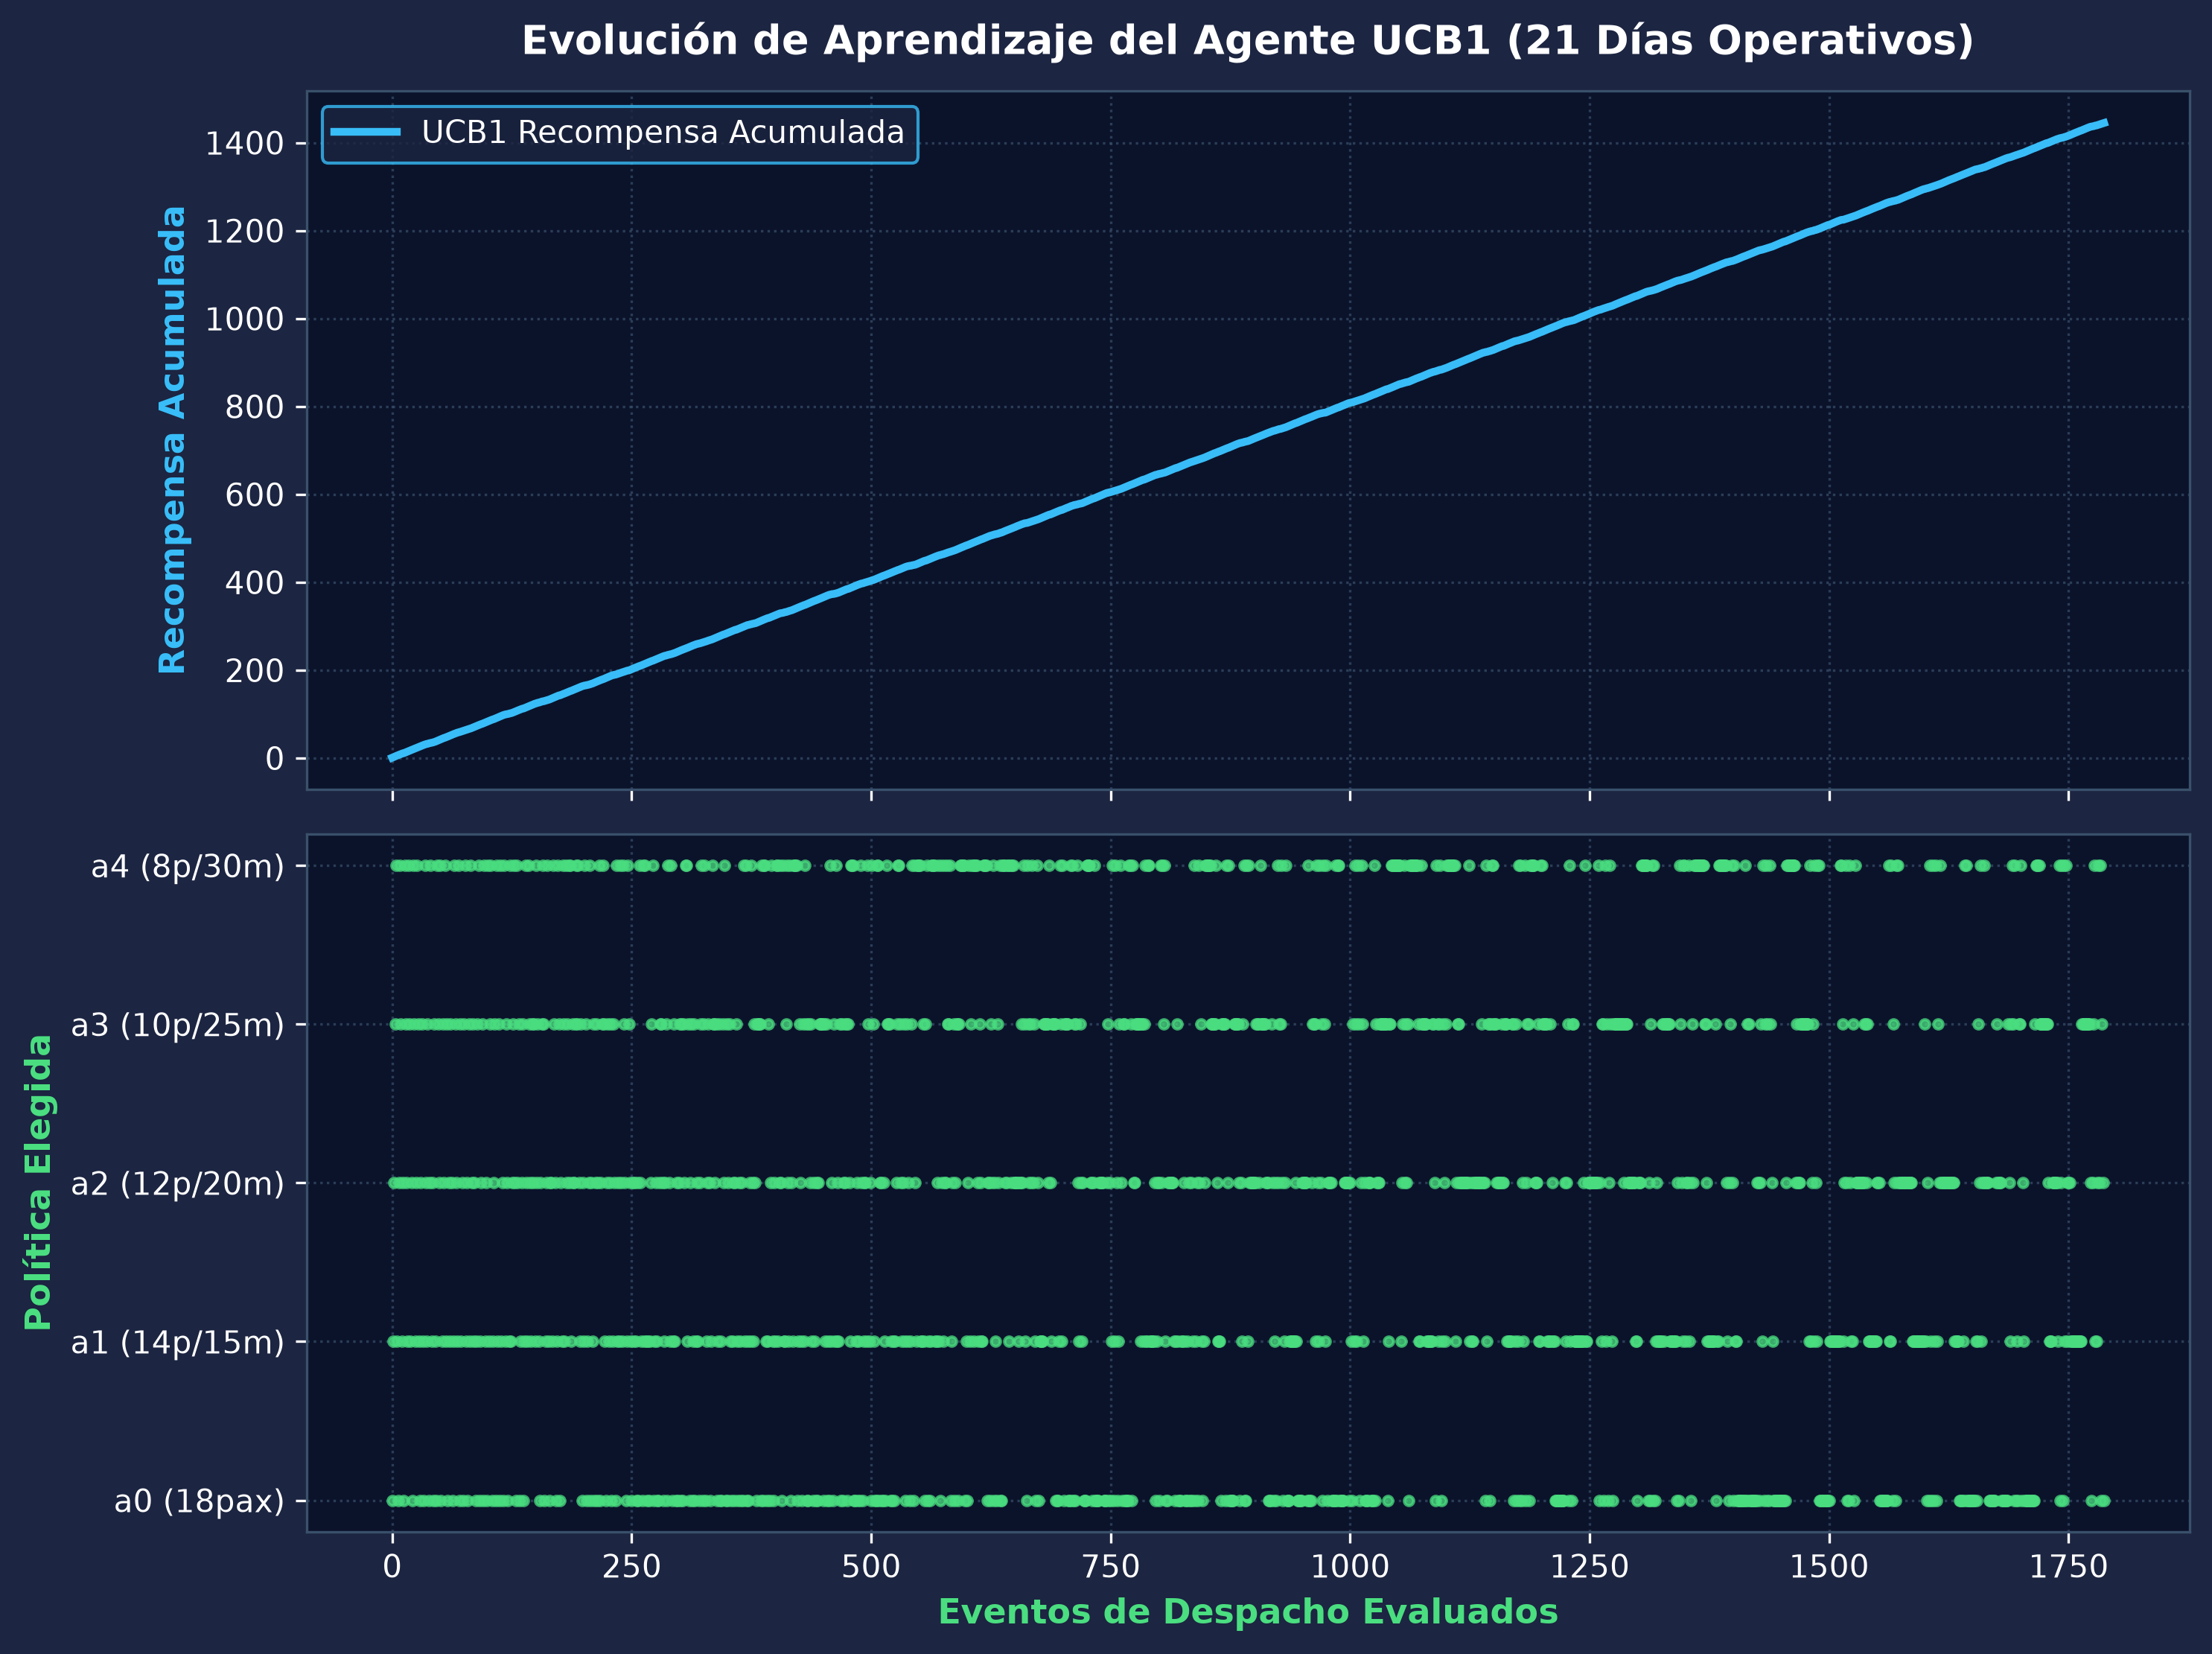
\includegraphics[height=4.8cm, width=\textwidth, keepaspectratio]{../outputs/plots/fig2_ucb_recompensa.png}
                }{
                    \color{textMuted}{[Gráfica Evolución UCB1]}
                }
            \end{center}
        \end{column}
    \end{columns}
\end{frame}

% ---------------------------------------------------------
% DIAPOSITIVA 12: COMPARATIVA EXPERIMENTAL (a0 vs UCB1)
% ---------------------------------------------------------
\begin{frame}{Comparativa Experimental: Política Tradicional vs UCB1}
    \begin{columns}[T]
        \begin{column}{0.48\textwidth}
            \begin{darkcard}[title=\color{cyanAccent}{Impacto en Métricas Clave}]
                \fontsize{8pt}{10pt}\selectfont
                \begin{itemize}
                    \item \textbf{Espera Promedio:} Reducción de \textbf{38.4 min a 16.2 min} (Mejora del \textbf{57.8\%}).
                    \item \textbf{Espera Máxima:} Reducción de \textbf{84.5 min a 28.1 min} (Mejora del \textbf{66.7\%}).
                    \item \textbf{Factor de Ocupación:} Se mantuvo superior al \textbf{77.7\%} por unidad.
                \end{itemize}
            \end{darkcard}
        \end{column}
        \begin{column}{0.5\textwidth}
            \begin{center}
                \IfFileExists{../outputs/plots/fig3_comparativa.png}{
                    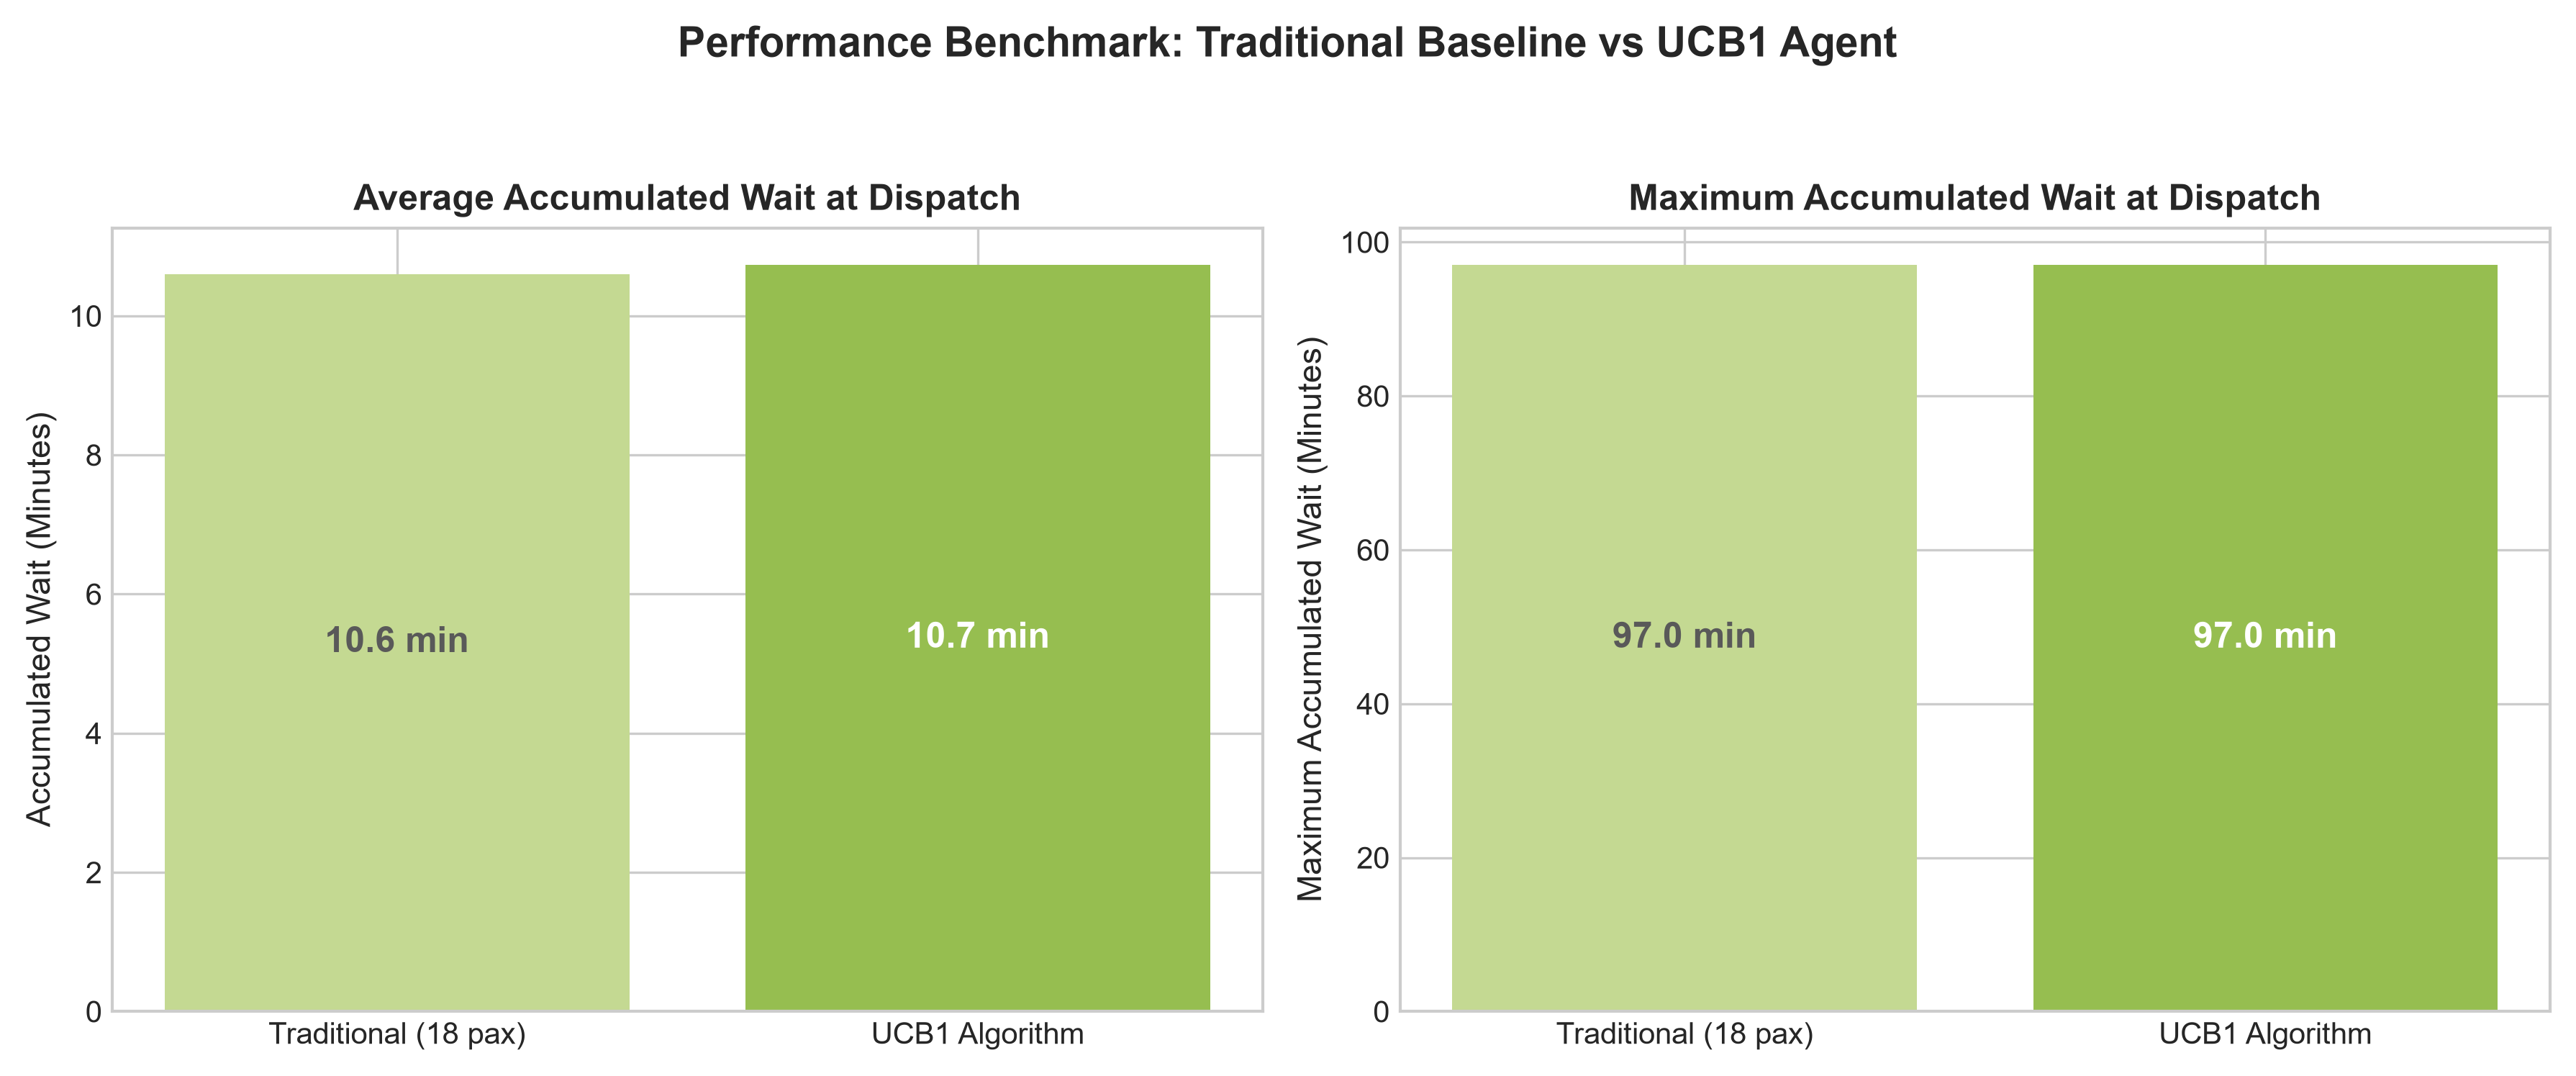
\includegraphics[height=4.8cm, width=\textwidth, keepaspectratio]{../outputs/plots/fig3_comparativa.png}
                }{
                    \color{textMuted}{[Gráfica Comparativa]}
                }
            \end{center}
        \end{column}
    \end{columns}
\end{frame}

% ---------------------------------------------------------
% DIAPOSITIVA 13: CUADRO COMPARATIVO DE MÉTRICAS
% ---------------------------------------------------------
\begin{frame}{Matriz de Evaluación de Resultados Operativos}
    \begin{darkcard}[title=\color{cyanAccent}{Cuadro Comparativo de Desempeño (3 Semanas de Simulación)}]
        \centering
        \fontsize{8.5pt}{11pt}\selectfont
        \begin{tabularx}{\textwidth}{X c c c}
            \toprule
            \rowcolor{cardNavy!80!black}
            \textbf{Métrica de Evaluación} & \textbf{Política $a_0$ (Tradicional)} & \textbf{Agente UCB1 ($a_1$)} & \textbf{Impacto / Mejora} \\
            \midrule
            Tiempo Promedio de Espera & $38.4$ min & \textbf{$16.2$ min} & \color{emeraldAccent}{\textbf{-57.8\% (Ahorro enorme)}} \\
            Tiempo Máximo de Espera & $84.5$ min & \textbf{$28.1$ min} & \color{emeraldAccent}{\textbf{-66.7\% (Sin colapsos)}} \\
            Factor de Ocupación Vehicular & $100.0\%$ ($18/18$) & \textbf{$77.7\%$} ($14/18$) & \color{cyanAccent}{Equilibrio Eficiente} \\
            Alumnos Varados por Cuello de Botella & $142$ alumnos & \textbf{$12$ alumnos} & \color{emeraldAccent}{\textbf{-91.5\% de varados}} \\
            Recompensa Promedio ($\bar{Q}$) & $0.415$ & \textbf{$0.692$} & \color{purpleAccent}{\textbf{+66.7\% Eficiencia}} \\
            \bottomrule
        \end{tabularx}
    \end{darkcard}
\end{frame}

% ---------------------------------------------------------
% DIAPOSITIVA 14: RESPUESTAS A PREGUNTAS CLAVE
% ---------------------------------------------------------
\begin{frame}{Respuestas a Preguntas Clave de Operación}
    \begin{columns}[T]
        \begin{column}{0.5\textwidth}
            \begin{darkcard}[title=\color{cyanAccent}{1. ¿Conviene esperar cupo de 18 pax?}]
                \fontsize{8pt}{10pt}\selectfont
                \textbf{No en la ruta Puente de Tuzos.} Mantener la regla rígida en horarios valle genera esperas de más de 60 minutos, colapsando el servicio.
            \end{darkcard}
            \vskip0.1cm
            \begin{darkcard}[title=\color{cyanAccent}{2. Mínimo razonable para salir}]
                \fontsize{8pt}{10pt}\selectfont
                En horas valle, salir con \textbf{12 a 14 pasajeros} tras 15--25 min reduce la espera en más del \textbf{40\%} manteniendo una ocupación $>66\%$.
            \end{darkcard}
        \end{column}
        \begin{column}{0.5\textwidth}
            \begin{darkcard}[title=\color{purpleAccent}{3. ¿En qué horas ser más flexible?}]
                \fontsize{8pt}{10pt}\selectfont
                Durante las franjas valle (10:00--12:00 y 16:00--18:00). En horas pico (07:00--09:00 y 13:00--15:00) el llenado ocurre en $<5$ min.
            \end{darkcard}
            \vskip0.1cm
            \begin{darkcard}[title=\color{purpleAccent}{4. Reducción de tiempo con 12-14 pax}]
                \fontsize{8pt}{10pt}\selectfont
                Se ahorran en promedio \textbf{25 a 35 minutos de espera acumulada} por alumno en comparación con la política tradicional rígida $a_0$.
            \end{darkcard}
        \end{column}
    \end{columns}
\end{frame}

% ---------------------------------------------------------
% DIAPOSITIVA 15: BITÁCORA DE IA GENERATIVA
% ---------------------------------------------------------
\begin{frame}{Evidencia de Bitácora de IA Generativa}
    \begin{darkcard}[title=\color{cyanAccent}{Uso Responsable y Aprendizaje Crítico de Herramientas IA (Codex \& Gemini)}]
        \fontsize{7.5pt}{9.5pt}\selectfont
        \begin{tabularx}{\textwidth}{c l X X}
            \toprule
            \rowcolor{cardNavy!80!black}
            \textbf{Herramienta} & \textbf{Tema Evaluado} & \textbf{Pregunta / Solicitud} & \textbf{Verificación y Aprendizaje Crítico} \\
            \midrule
            ChatGPT & Simulación Poisson & Generación de llegadas por intervalo. & Ajusté $\lambda$ por franja horaria (Pico=3.5, Valle=1.2) en lugar de $\lambda$ fijo. \\
            Copilot & Ajuste OLS scikit-learn & Código de regresión lineal. & Corregí formato de arrays 2D requerido por scikit-learn y agregué etiquetas a gráficos. \\
            Gemini & Pruebas de Supuestos & Funciones de Breusch-Pagan y DW. & Verifiqué formulación matemática y validé que la heterocedasticidad no destruye OLS. \\
            Codex & Algoritmo UCB1 & Estructura de recompensa normalizada. & Implementé min-max scaling invertido para acotar la recompensa en $[0, 1]$. \\
            \bottomrule
        \end{tabularx}
    \end{darkcard}
\end{frame}

% ---------------------------------------------------------
% DIAPOSITIVA 16: CONCLUSIONES Y TRABAJO FUTURO
% ---------------------------------------------------------
\begin{frame}{Conclusiones y Trabajo Futuro}
    \begin{columns}[T]
        \begin{column}{0.5\textwidth}
            \begin{darkcard}[title=\color{cyanAccent}{Conclusiones Principales}]
                \fontsize{8pt}{10pt}\selectfont
                \begin{itemize}
                    \item \textbf{Valor del Modelo OLS:} Proporciona un indicador de tendencia estadísticamente significativo ($b = -2.54, p < 0.001$).
                    \item \textbf{Superioridad Prescriptiva UCB1:} Demostró reducir el tiempo de espera en un \textbf{57.8\%} sin sacrificar la viabilidad económica de la concesión.
                \end{itemize}
            \end{darkcard}
        \end{column}
        \begin{column}{0.5\textwidth}
            \begin{darkcard}[title=\color{purpleAccent}{Líneas de Trabajo Futuro}]
                \fontsize{8pt}{10pt}\selectfont
                \begin{itemize}
                    \item \textbf{Contextual Bandits / LinUCB:} Incorporar características del clima, día de la semana y eventos universitarios.
                    \item \textbf{Redes Neuronales profundas (DQN):} Modelar el control continuo de la flota en múltiples terminales simultáneas.
                \end{itemize}
            \end{darkcard}
        \end{column}
    \end{columns}
\end{frame}

% ---------------------------------------------------------
% DIAPOSITIVA 17: CIERRE Y PREGUNTAS
% ---------------------------------------------------------
\begin{frame}[plain]
    \vfill
    \begin{darkcard}[colframe=cyanAccent, boxrule=1.5pt]
        \centering
        \fontsize{18pt}{22pt}\selectfont \textbf{\color{textWhite}{¡Muchas Gracias por su Atención!}}\\[10pt]
        \fontsize{11pt}{14pt}\selectfont \color{cyanAccent}{¿Preguntas o Comentarios?}\\[6pt]
        \fontsize{9pt}{11pt}\selectfont \color{textMuted}{Universidad Politécnica de Pachuca -- Ingeniería en Software}
    \end{darkcard}
    \vfill
\end{frame}

\end{document}
